The feature is realized in the following function
\begin{lstlisting}
  void ghost_removal(const vector<Mat>& pics, int iter, vector<Mat>& result)
\end{lstlisting}
which is an implementation of \textbf{EA Khan's method} \cite{ref:ghost-removal}. The algorithm iteratively calculate the possibility of each pixel based on its weight, and then calculate the weight for the next iteration by its possibility. For a series of $R$ photos under different exposure times, we assign a vector $\textbf{x}_{ijr}=(L, a, b, i, j)\in \mathbb{R}^5$ to each pixel on a photo, where $L$, $a$, $b$ represent its color, $i$, $j$ represent its position, and $r$ represents the number of photo that contains it. Define the neighborhood of the vector $\textbf{x}_{ijr}$
$$F=\{ \textbf{y}_{pqs}|(p,q,s)\in\textbf{N}(\textbf{x}_{ijr}), (p,q)\neq(i,j), s=1,2,\cdots,R \}$$
In the first iteration, define the weight by a hat function (Fig. \ref{fig:hat})
$$w(Z)=1-\left(2\cdot\frac{Z}{255}-1\right)^{12}$$

\begin{figure}[!ht]
\center
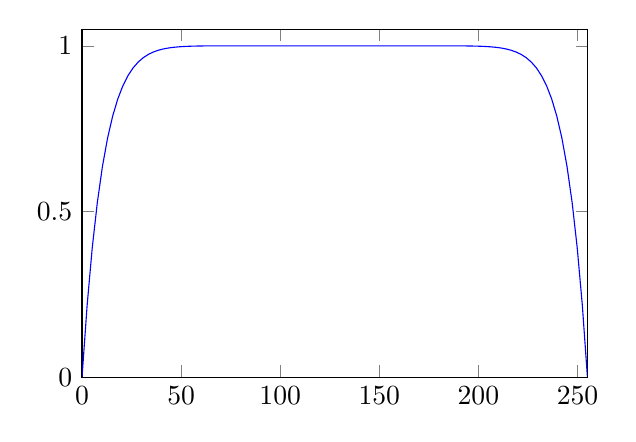
\begin{tikzpicture}
  \begin{axis}[
    domain=0:255,
    xmin=0, xmax=255,
    ymin=0, ymax=1.05,
    samples=100,
    width=8cm, height=6cm
  ]
    \addplot+[mark=none] {1-(2*(x/255)-1)^12};
  \end{axis}
\end{tikzpicture}
\caption{Hat function for ghost removal weighting}
\label{fig:hat}
\end{figure}

where $Z$ is the average value of three channels. Then, calculate the possibility by
$$ 
P(\textbf{x}_{ijr}|F)=
\frac{
  \sum_{p,q,s\in N(\textbf{x}_{ijr})}w_{pqs}K_\textbf{H}(\textbf{x}_{ijr}-\textbf{y}_{pqs})
  }{
    \sum_{p,q,s\in N(\textbf{x}_{ijr})}w_{pqs}
  } 
$$
where
$$K_\textbf{H}(\textbf{x})=|\textbf{H}|^{-1/2}(2\pi)^{-5/2}\exp(-\frac{1}{2}\textbf{x}^T\textbf{H}^{-1}\textbf{x})$$
and $\textbf{H}$ is an identity matrix. Afterwards, calculate the weight for the next iteration
$$w_{pqs, t+1}=w(Z_s(p,q))\cdot P(\textbf{x}_{ijr}|F)$$
in which $w(Z_s(p,q))$ stands for the initial weight.

